\section{The chain rule} \label{S:2.5.Chain}

\vspace*{-14 pt}
\framebox{\hspace*{3 pt}
\parbox{\boxwidth}{\begin{goals}
\item What is a composite function and how do we recognize its structure algebraically?
\item Given a composite function $C(x) = f(g(x))$ that is built from differentiable functions $f$ and $g$, how do we compute $C'(x)$ in terms of $f$, $g$, $f'$, and $g'$?  What is the statement of the Chain Rule?
\end{goals}} \hspace*{3 pt}}

\subsection*{Introduction}

In addition to learning how to differentiate a variety of basic functions, we have also been developing our ability to understand how to use rules to differentiate certain algebraic combinations of them.  For example, we not only know how to take the derivative of $f(x) = \sin(x)$ and $g(x) = x^2$, but now we can quickly find the derivative of each of the following combinations of $f$ and $g$:
$$s(x) = 3x^2 - 5\sin(x),$$
$$p(x) = x^2 \sin(x), \mbox{and}$$
$$q(x) = \frac{\sin(x)}{x^2}.$$
Finding $s'$ uses the sum and constant multiple rules, determining $p'$ requires the product rule, and $q'$ can be attained with the quotient rule.  Again, we note the importance of recognizing the algebraic structure of a given function in order to find its derivative:  $s(x) = 3g(x) - 5f(x)$, $p(x) = g(x) \cdot f(x)$, and $q(x) =\frac{f(x)}{g(x)}.$

There is one more natural way to algebraically combine basic functions, and that is by \emph{composing} them.  For instance, let's consider the function
$$C(x) = \sin(x^2),$$
and observe that any input $x$ passes through a \emph{chain} of functions.  In particular, in the process that defines the  function $C(x)$, $x$ is first squared, and then the sine of the result is taken.  Using an arrow diagram,
$$x \longrightarrow x^2 \longrightarrow \sin(x^2).$$
In terms of the elementary functions $f$ and $g$, we observe that $x$ is first input in the function $g$, and then the result is used as the input in $f$.  Said differently, we can write
$$C(x) = f(g(x)) = \sin(x^2)$$
and say that $C$ is the \emph{composition} \index{composition} of $f$ and $g$.  We will refer to $g$, the function that is first applied to $x$, as the \emph{inner} function, while $f$, the function that is applied to the result, is the \emph{outer} function.

The main question that we answer in the present section is: given a composite function $C(x) = f(g(x))$ that is built from differentiable functions $f$ and $g$, how do we compute $C'(x)$ in terms of $f$, $g$, $f'$, and $g'$?  In the same way that the rate of change of a product of two functions, $p(x) = f(x) \cdot g(x)$, depends on the behavior of both $f$ and $g$, it makes sense intuitively that the rate of change of a composite function $C(x) = f(g(x))$ will also depend on some combination of $f$ and $g$ and their derivatives.  The rule that describes how to compute $C'$ in terms of $f$ and $g$ and their derivatives will be called the \emph{chain rule}.

But before we can learn what the chain rule says and why it works, we first need to be comfortable decomposing composite functions so that we can correctly identify the inner and outer functions, as we did in the example above with $C(x) = \sin(x^2).$ 

\begin{pa} \label{PA:2.5}
For each function given below, identify its fundamental algebraic structure.  In particular, is the given function a sum, product, quotient, or composition of basic functions?  If the function is a composition of basic functions, state a formula for the inner function $g$ and the outer function $f$ so that the overall composite function can be written in the form $f(g(x))$.  If the function is a sum, product, or quotient of basic functions, use the appropriate rule to determine its derivative. 
\ba
	\item $h(x) = \tan(2^x)$
	\item $p(x) = 2^x \tan(x)$
	\item $r(x) = (\tan(x))^2$
	\item $m(x) = e^{\tan(x)}$
	\item $w(x) = \sqrt{x} + \tan(x)$
	\item $z(x) = \sqrt{\tan(x)}$
\ea
\end{pa} 
\afterpa

\subsection*{The chain rule}

One of the challenges of differentiating a composite function is that it often cannot be written in an alternate algebraic form.  For instance, the function $C(x) = \sin(x^2)$ cannot be expanded or otherwise rewritten, so it presents no alternate approaches to taking the derivative.  But other composite functions can be expanded or simplified, and these present a way to begin to explore how the chain rule might have to work.  To that end, we consider two examples of composite functions that present alternate means of finding the derivative.

\bex \label{Ex:2.5.Linear}
Let $f(x) = -4x + 7$ and $g(x) = 3x - 5$.  Determine a formula for $C(x) = f(g(x))$ and compute $C'(x)$.  How is $C'$ related to $f$ and $g$ and their derivatives?
\eex
By the rules given for $f$ and $g$, 
\begin{eqnarray*}
C(x) & = & f(g(x)) \\
       & = & f(3x-5) \\
       & = & -4(3x-5) + 7 \\
       & = & -12x + 20 + 7 \\
       & = & -12x + 27.
\end{eqnarray*}
Thus, $C'(x) = -12$.  Noting that $f'(x) = -4$ and $g'(x) = 3$, we observe that $C'$ appears to be the product of $f'$ and $g'$.
\afterex
From one perspective, Example~\ref{Ex:2.5.Linear} may be too elementary.  Linear functions are the simplest of all functions, and perhaps composing linear functions (which yields another linear function) does not exemplify the true complexity that is involved with differentiating a composition of more complicated functions.  At the same time, we should remember the perspective that any differentiable function is \emph{locally} linear, so any function with a derivative behaves like a line when viewed up close.  From this point of view, the fact that the derivatives of $f$ and $g$ are multiplied to find the derivative of their composition turns out to be a key insight.

We now consider a second example involving a nonlinear function to gain further understanding of how differentiating a composite function involves the basic functions that combine to form it.

\bex \label{Ex:2.5.DoubleAngle}
Let $C(x) = \sin(2x).$  Use the double angle identity to rewrite $C$ as a product of basic functions, and use the product rule to find $C'$.  Rewrite $C'$ in the simplest form possible.  
\eex
By the double angle identity for the sine function,
$$C(x) = \sin(2x) = 2\sin(x)\cos(x).$$
Applying the product rule and simplifying,
$$C'(x) = 2\sin(x)(-\sin(x)) + \cos(x)(2\cos(x)) = 2(\cos^2(x) - \sin^2(x)).$$
Next, we recall that one of the double angle identities for the cosine function tells us that 
$$\cos(2x) = \cos^2(x) - \sin^2(x).$$
Substituting this result in our expression for $C'(x)$, we now have that
$$C'(x) = 2 \cos(2x).$$
\afterex
So from Example~\ref{Ex:2.5.DoubleAngle}, we see that if $C(x) = \sin(2x)$, then $C'(x) = 2\cos(2x)$.  Letting $g(x) = 2x$ and $f(x) = \sin(x)$, we observe that $C(x) = f(g(x))$.  Moreover, with $g'(x) = 2$ and $f'(x) = \cos(x)$, it follows that we can view the structure of $C'(x)$ as
$$C'(x) = 2\cos(2x) = g'(x) f'(g(x)).$$
In this example, we see that for the composite function $C(x) = f(g(x))$, the derivative $C'$ is (as in the example involving linear functions) constituted by multiplying the derivatives of $f$ and $g$, but with the special condition that $f'$ is evaluated at $g(x)$, rather than at $x$.

It makes sense intuitively that these two quantities are involved in understanding the rate of change of a composite function:  if we are considering $C(x) = f(g(x))$ and asking how fast $C$ is changing at a given $x$ value as $x$ changes, it clearly matters (a) how fast $g$ is changing at $x$, as well as how fast $f$ is changing at the value of $g(x)$.  It turns out that this structure holds not only for the functions in Examples~\ref{Ex:2.5.Linear} and~\ref{Ex:2.5.DoubleAngle}, but indeed for all differentiable functions\footnote{Like other differentiation rules, the Chain Rule can be proved formally using the limit definition of the derivative.} as is stated in the Chain Rule.

\vspace*{5pt}
\nin \framebox{\hspace*{3 pt}
\parbox{\boxwidth}{
{\bf Chain Rule:} \index{chain rule} If $g$ is differentiable at $x$ and $f$ is differentiable at $g(x)$, then the composite function $C$ defined by $C(x) = f(g(x))$ is differentiable at $x$ and  
$$C'(x) = f'(g(x)) g'(x).$$
} \hspace*{3 pt}}
\vspace*{1pt}

As with the product and quotient rules, it is often helpful to think verbally about what the chain rule says: ``If $C$ is a composite function defined by an outer function $f$ and an inner function $g$, then $C'$ is given by the derivative of the outer function, evaluated at the inner function, times the derivative of the inner function.''  

At least initially in working particular examples requiring the chain rule, it can also be helpful to clearly identify the inner function $g$ and outer function $f$, compute their derivatives individually, and then put all of the pieces together to generate the derivative of the overall composite function.  To see what we mean by this, consider the function
$$r(x) = (\tan(x))^2.$$
The function $r$ is composite, with inner function $g(x) = \tan(x)$ and outer function $f(x) = x^2$.  Organizing the key information involving $f$, $g$, and their derivatives, we have

\begin{center}
\begin{tabular}{lcl}
$f(x) = x^2$ & \hspace{0.5in} & $g(x) = \tan(x)$ \\
$f'(x) = 2x$ & \hspace{0.5in} & $g'(x) = \sec^2(x)$ \\
$f'(g(x)) = 2\tan(x)$ & \hspace{0.5in} & \ \\
\end{tabular}
\end{center}

Applying the chain rule, which tells us that $r'(x) = f'(g(x)) g'(x)$, we find that for $r(x) = (\tan(x))^2$, its derivative is
$$r'(x) = 2\tan(x) \sec^2(x).$$

As a side note, we remark that another way to write $r(x)$ is $r(x) = \tan^2(x)$.  Observe that in this format, the composite nature of the function is more implicit, but this is common notation for powers of trigonometric functions:  $\cos^4(x)$, $\sin^5(x)$, and $\sec^2(x)$ are all composite functions, with the outer function a power function and the inner function a trigonometric one.

The chain rule now substantially expands the library of functions we can differentiate, as the following activity demonstrates.

\begin{activity} \label{A:2.5.1}  
For each function given below, identify an inner function $g$ and outer function $f$ to write the function in the form $f(g(x))$.  Then, determine $f'(x)$, $g'(x)$, and $f'(g(x))$, and finally apply the chain rule to determine the derivative of the given function.  
\ba
	   \item $h(x) = \cos(x^4)$
	   \item  $p(x) = \sqrt{ \tan(x) }$
           \item $s(x) = 2^{\sin(x)}$
           \item $z(x) = \cot^5(x)$
           \item $m(x) = (\sec(x) + e^x)^9$
\ea
\end{activity}
\begin{smallhint}
\ba
	   \item The outer function is $f(x) = \cos(x)$.
	   \item The outer function is $f(x) = \sqrt{x}$.
           \item The outer function is $f(x) = 2^x$.
           \item The outer function is $f(x) = x^5$.
           \item The outer function is $f(x) = x^9$.
\ea
\end{smallhint}
\begin{bighint}
\ba
	   \item The outer function is $f(x) = \cos(x)$, while the inner function is $g(x) = x^4$.
	   \item The outer function is $f(x) = \sqrt{x}$, while the inner function is $g(x) = \tan(x)$.
           \item The outer function is $f(x) = 2^x$, while the inner function is $g(x) = \sin(x)$.
           \item The outer function is $f(x) = x^5$, while the inner function is $g(x) = \cot(x)$.
           \item The outer function is $f(x) = x^9$, while the inner function is $g(x) = \sec(x) + e^x$.
\ea
\end{bighint}
\begin{activitySolution}
\ba
	   \item The outer function is $f(x) = \cos(x)$, while the inner function is $g(x) = x^4$, and we know that 
	   $$f'(x) = -\sin(x), g'(x) = 4x^3, \ \mbox{and} \ f'(g(x)) = -\sin(x^4).$$
	   Hence, by the chain rule,
	   $$h'(x) = f'(g(x))g'(x) = -4x^3\sin(x^4).$$
	   \item The outer function is $f(x) = \sqrt{x}$, while the inner function is $g(x) = \tan(x)$, and we know that 
	   $$f'(x) = \frac{1}{2\sqrt{x}}, g'(x) = \sec^2(x), \ \mbox{and} \ f'(g(x)) = \frac{1}{2\sqrt{\tan(x)}}.$$
	   Hence, by the chain rule,
	   $$h'(x) = f'(g(x))g'(x) = \frac{\sec^2(x)}{2\sqrt{\tan(x)}}.$$
           \item The outer function is $f(x) = 2^x$, while the inner function is $g(x) = \sin(x)$, and we know that 
	   $$f'(x) = 2^x \ln(2), g'(x) = \cos(x), \ \mbox{and} \ f'(g(x)) = 2^{\sin(x)}\ln(2).$$
	   Hence, by the chain rule,
	   $$h'(x) = f'(g(x))g'(x) = 2^{\sin(x)}\ln(2)\cos(x).$$
           \item The outer function is $f(x) = x^5$, while the inner function is $g(x) = \cot(x)$, and we know that 
	   $$f'(x) = 5x^4, g'(x) = -\csc^2(x), \ \mbox{and} \ f'(g(x)) = 5\cot^4(x).$$
	   Hence, by the chain rule,
	   $$h'(x) = f'(g(x))g'(x) = -5\cot^4(x) \csc^2(x).$$
           \item The outer function is $f(x) = x^9$, while the inner function is $g(x) = \sec(x) + e^x$, and we know that 
	   $$f'(x) = 9x^8, g'(x) = \sec(x)\tan(x) + e^x, \ \mbox{and} \ f'(g(x)) = 9(\sec(x)+e^x)^8.$$
	   Hence, by the chain rule,
	   $$h'(x) = f'(g(x))g'(x) = 9(\sec(x)+e^x)^8 (\sec(x)\tan(x) + e^x).$$
\ea
\end{activitySolution}
\aftera

\subsection*{Using multiple rules simultaneously}

The chain rule now joins the sum, constant multiple, product, and quotient rules in our collection of the different techniques for finding the derivative of a function through understanding its algebraic structure and the basic functions that constitute it.  It takes substantial practice to get comfortable with navigating multiple rules in a single problem; using proper notation and taking a few extra steps can be particularly helpful as well.  We demonstrate with an example and then provide further opportunity for practice in the following activity.

\bex
Find a formula for the derivative of $h(t) = 3^{t^2 + 2t}\sec^4(t)$. 
\eex
We first observe that the most basic structure of $h$ is that it is the product of two functions:  $h(t) = a(t) \cdot b(t)$ where $a(t) = 3^{t^2 + 2t}$ and $b(t) = \sec^4(t)$.  Therefore, we see that we will need to use the product rule to differentiate $h$.  When it comes time to differentiate $a$ and $b$ in their roles in the product rule, we observe that since each is a composite function, the chain rule will be needed.  We therefore begin by working separately to compute $a'(t)$ and $b'(t)$.

Writing $a(t) = f(g(t)) = 3^{t^2 + 2t}$, and finding the derivatives of $f$ and $g$, we have
\begin{center}
\begin{tabular}{lcl}
$f(t) = 3^t$ & \hspace{0.5in} & $g(t) = t^2 + 2t$ \\
$f'(t) = 3^t \ln(3)$ & \hspace{0.5in} & $g'(t) = 2t+1$ \\
$f'(g(t)) = 3^{t^2 + 2t}\ln(3)$ & \hspace{0.5in} & \ \\
\end{tabular}
\end{center}
Thus, by the chain rule, it follows that $a'(t) = f'(g(t))g'(t) = 3^{t^2 + 2t}\ln(3) (2t+1).$

Turning next to $b$, we write $b(t) = r(s(t)) = \sec^4(t)$ and find the derivatives of $r$ and $g$.  Doing so, 
\begin{center}
\begin{tabular}{lcl}
$r(t) = t^4$ & \hspace{0.5in} & $s(t) = \sec(t)$ \\
$r'(t) = 4t^3$ & \hspace{0.5in} & $s'(t) = \sec(t)\tan(t)$ \\
$r'(s(t)) = 4\sec^3(t)$ & \hspace{0.5in} & \ \\
\end{tabular}
\end{center}
By the chain rule, we now know that $b'(t) = r'(s(t))s'(t) = 4\sec^3(t)\sec(t)\tan(t) = 4 \sec^4(t) \tan(t).$

Now we are finally ready to compute the derivative of the overall function $h$.  Recalling that $h(t) = 3^{t^2 + 2t}\sec^4(t)$, by the product rule we have
$$h'(t) = 3^{t^2 + 2t} \frac{d}{dt}[\sec^4(t)] + \sec^4(t) \frac{d}{dt}[3^{t^2 + 2t}].$$
From our work above with $a$ and $b$, we know the derivatives of $3^{t^2 + 2t}$ and $\sec^4(t)$, and therefore
$$h'(t) = 3^{t^2 + 2t} 4\sec^4(t) \tan(t) + \sec^4(t) 3^{t^2 + 2t}\ln(3) (2t+2).$$
\afterex

\begin{activity} \label{A:2.5.2}  
For each of the following functions, find the function's derivative.  State the rule(s) you use, label relevant derivatives appropriately, and be sure to clearly identify your overall answer.  
\ba
	\item $p(r) = 4\sqrt{r^6 + 2e^r}$
	\item $m(v) = \sin(v^2) \cos(v^3)$
	\item $\ds h(y) = \frac{\cos(10y)}{e^{4y}+1}$
	\item $s(z) = 2^{z^2 \sec (z)}$
	\item $\ds c(x) = \sin(e^{x^2})$
\ea
\end{activity}
\begin{smallhint}
\ba
	\item Use the constant multiple rule first, followed by the chain rule.
	\item Observe that $m$ is fundamentally a product of composite functions.
	\item Note that $h$ is a quotient of composite functions.
	\item The function $s$ is a composite function with outer function $2^z$.
	\item It is possible for a function to be a composite function with more than two functions in the chain.
\ea
\end{smallhint}
\begin{bighint}
\ba
	\item Note that $p'(r) = 4\frac{d}{dr}[\sqrt{r^6 + 2e^r}].$  Now use the chain rule to complete the remaining derivative.
	\item Observe that by the product rule, $m'(v) = \sin(v^2) \frac{d}{dv}[\cos(v^3)] + \cos(v^3) \frac{d}{dv}[\sin(v^2)].$  What rule is needed to execute the remaining two derivatives?
	\item Note that by the quotient rule,
	$$h'(y) = \frac{(e^{4y}+1) \frac{d}{dy}[\cos(10y)] - \cos(10y) \frac{d}{dy}[e^{4y}+1]}{(e^{4y}+1)^2}.$$
	What work remains to find $h'(y)$?
	\item By the chain rule, $s'(z) = 2^{z^2\sec(z)} \ln(2) \frac{d}{dz}[z^2 \sec(z)]$.  What rule should next be applied?
	\item If we first apply the chain rule to the outer function (the sine function), note that 
	$$c'(x) = \cos(e^{x^2}) \frac{d}{dx}[e^{x^2}].$$
	What rule is needed to differentiate the inner function, $e^{x^2}$?
\ea
\end{bighint}
\begin{activitySolution}
\ba
	\item By the constant multiple rule, $p'(r) = 4\frac{d}{dr}[\sqrt{r^6 + 2e^r}].$  Using the chain rule to complete the remaining derivative, we see that
	$$p'(r) = 4 \frac{1}{2\sqrt{r^6 + 2e^r}} \frac{d}{dr}[r^6 + 2e^r] = \frac{4(6r^5 + 2e^r)}{2\sqrt{r^6 + 2e^r}}.$$
	\item Observe that by the product rule, $m'(v) = \sin(v^2) \frac{d}{dv}[\cos(v^3)] + \cos(v^3) \frac{d}{dv}[\sin(v^2)].$  Applying the chain rule to differentiate $\cos(v^3)$ and $\sin(v^2)$, we see that 
	$$m'(v) = \sin(v^2) [-\sin(v^3) \cdot 3v^2] + \cos(v^3) [\cos(v^2) \cdot 2v] = -3v^2 \sin(v^2)\sin(v^3) + 2v \cos(v^3)\cos(v^2).$$ 
	\item By the quotient rule,
	$$h'(y) = \frac{(e^{4y}+1) \frac{d}{dy}[\cos(10y)] - \cos(10y) \frac{d}{dy}[e^{4y}+1]}{(e^{4y}+1)^2}.$$
	Applying the chain rule to differentiate $\cos(10y)$ and $e^{4y}$, it follows
	$$h'(y) = \frac{(e^{4y}+1) [-10\sin(10y)] - \cos(10y) [4e^{4y}]}{(e^{4y}+1)^2}.$$
	\item By the chain rule, $s'(z) = 2^{z^2\sec(z)} \ln(2) \frac{d}{dz}[z^2 \sec(z)]$.  Then by the product rule, we find that
	$$s'(z) = 2^{z^2\sec(z)} \ln(2) [z^2 \sec(z)\tan(z) + \sec(z) \cdot 2z].$$
	\item If we first apply the chain rule to the outer function (the sine function), note that 
	$$c'(x) = \cos(e^{x^2}) \frac{d}{dx}[e^{x^2}].$$
	Next, we again apply the chain rule, but this time to $e^{x^2}$, and get
	$$c'(x) = \cos(e^{x^2}) [e^{x^2}\cdot 2x].$$
\ea
\end{activitySolution}
\aftera

The chain rule now adds substantially to our ability to do different familiar problems that involve derivatives.  Whether finding the equation of the tangent line to a curve, the instantaneous velocity of a moving particle, or the instantaneous rate of change of a certain quantity, if the function under consideration involves a composition of other functions, the chain rule is indispensable.

\begin{activity} \label{A:2.5.3}   Use known derivative rules, including the chain rule, as needed to answer each of the following questions.
\ba
	\item Find an equation for the tangent line to the curve $y= \sqrt{e^x + 3}$ at the point where $x=0$.

  	\item If $\displaystyle s(t) = \frac{1}{(t^2+1)^3}$ represents the position function of a particle moving horizontally along an axis at time $t$ (where $s$ is measured in inches and $t$ in seconds), find the particle's instantaneous velocity at $t=1$.  Is the particle moving to the left or right at that instant?

  	\item At sea level, air pressure is 30 inches of mercury.  At an altitude of $h$ feet above sea level, the air pressure, $P$, in inches of mercury, is given by the function
$$P = 30 e^{-0.0000323 h}.$$
Compute $dP/dh$ and explain what this derivative function tells you about air pressure, including a discussion of the units on $dP/dh$.  In addition, determine how fast the air pressure is changing for a pilot of a small plane passing through an altitude of $1000$ feet.
  	
	\item Suppose that $f(x)$ and $g(x)$ are differentiable functions and that the following information about them is known:
	
\begin{center}
\begin{tabular}{ | c | c | c | c | c | }
   \hline 
   $x$ 	& $f(x)$  	& $f'(x)$	& $g(x)$	& $g'(x)$ \\  \hline

   $-1$ 	& $2$	& $-5$ & $-3$ &  $4$ \\ \hline

   $2$ 	& $-3$	& $4$ & $-1$ &  $2$ \\ \hline
\end{tabular}
\end{center}

If $C(x)$ is a function given by the formula $f(g(x))$, determine $C'(2)$.   In addition, if $D(x)$ is the function $f(f(x))$, find $D'(-1)$. 
\ea
\end{activity}
\begin{smallhint}
\ba
	\item Let $f(x) = \sqrt{e^x + 3}.$ Find $f'(x)$ and $f'(0)$.
  	\item Recall that $s'(t)$ tells us the instantaneous velocity at time $t$.
  	\item Note that the units on $dP/dh$ are inches of mercury per foot.
  	\item Since $C(x) = f(g(x)),$ it follows $C'(x) = f'(g(x))g'(x).$  What is $C'(2)$?
\ea
\end{smallhint}
\begin{bighint}
\ba
	\item Let $f(x) = \sqrt{e^x + 3}.$ Find $f'(x)$ and $f'(0)$ and recall the point-slope form of the tangent line.
  	\item Recall that $s'(t)$ tells us the instantaneous velocity at time $t$.  Consider writing $s(t) = (t^2 + 1)^{-3}$ for ease of differentiation.
  	\item Note that the units on $dP/dh$ are inches of mercury per foot so this derivative measures the instantaneous rate of change of barometric pressure with respect to elevation.  
  	\item Since $C(x) = f(g(x)),$ it follows $C'(x) = f'(g(x))g'(x).$  What is $C'(2)$?  What does the chain rule tell us about $\frac{d}{dx}[f(f(x))]$?
\ea
\end{bighint}
\begin{activitySolution}
\ba
	\item Let $f(x) = \sqrt{e^x + 3}.$ By the chain rule $f'(x) = \frac{e^x}{2\sqrt{e^x + 3}}$, and thus $f'(0) = \frac{1}{4}$.  Note further that $f(0) = \sqrt{1 + 3} = 2$.  The tangent line is therefore the line through $(0,2)$ with slope $1/4$, which is
	$$y - 2 = \frac{1}{4}(x-0).$$
  	\item Observe that $s(t) = (t^2 + 1)^{-3}$, and thus by the chain rule, $s'(t) = -3(t^2 + 1)^{-4}(2t).$  We therefore see that $s'(1) = -\frac{6}{16} = -\frac{3}{8}$ inches per second, so the particle is moving left at the instant $t = 1$.
  	\item First, $P'(h) = \frac{dP}{dh} = 30 e^{-0.0000323h} (-0.0000323).$  Therefore, $P'(1000) = 30 e^{-0.0323} (-0.0000323) \approx -0.000938$ inches of mercury per foot.  This tells us that the barometric pressure is dropping very slightly for each additional foot of elevation gaine.
	  
  	\item Since $C(x) = f(g(x)),$ it follows $C'(x) = f'(g(x))g'(x).$  Therefore, $C'(2) = f'(g(2))g'(2)$.  From the given table, $g(2) = -1$, so applying this result and using additional given information,
	$$C'(2) = f'(-1) g'(2) = (-5)(2) = -10.$$  
	For $D(x) = f(f(x))$, the chain rule tells us that $D'(x) = f'(f(x))f'(x)$, so $D'(-1) = f'(f(-1))f'(-1)$.  Using the given table, it follows
	$$D'(-1) = f'(2)f'(-1) = (4)(-5) = -20.$$ 
\ea
\end{activitySolution}
\aftera

\subsection*{The composite version of basic function rules}

As we gain more experience with differentiating complicated functions, we will become more comfortable in the process of simply writing down the derivative without taking multiple steps.  We demonstrate part of this perspective here by showing how we can find a composite rule that corresponds to two of our basic functions.  For instance, we know that $\frac{d}{dx}[\sin(x)] = \cos(x)$.  If we instead want to know
$$\frac{d}{dx}[\sin(u(x))],$$
where $u$ is a differentiable function of $x$, then this requires the chain rule with the sine function as the outer function.  Applying the chain rule,
$$\frac{d}{dx}[\sin(u(x))] = \cos(u(x)) \cdot u'(x).$$
Similarly, since $\frac{d}{dx}[a^x] = a^x \ln(a)$, it follows by the chain rule that 
$$\frac{d}{dx}[a^{u(x)}] = a^{u(x)} \ln(a) \cdot u'(x).$$
In the process of getting comfortable with derivative rules, an excellent exercise is to write down a list of all basic functions whose derivatives are known, list those derivatives, and then write the corresponding chain rule for the composite version with the inner function being an unknown function $u(x)$ and the outer function being the known basic function.  These versions of the chain rule are particularly simple when the inner function is linear, since the derivative of a linear function is a constant.  For instance,
$$\frac{d}{dx} \left[ (5x+7)^{10} \right] = 10(5x+7)^9 \cdot 5,$$
$$\frac{d}{dx} \left[ \tan(17x) \right] = 17\sec^2(17x), \ \mbox{and}$$
$$\frac{d}{dx} \left[ e^{-3x} \right] = -3e^{-3x}.$$
%\begin{center}
%\begin{tabular}{|l|r||l|r|}
%\hline
%$f(x)$ & $\frac{d}{dx}[f(x)]$ & $f(u(x))$ & $\frac{d}{dx}[f(u(x))]$ \\
%\hline 
%\hline
%$x^n$ & $nx^{n-1}$  & $[u(x)]^n$ & $n[u(x)]^{n-1} u'(x)$ \\
%\hline
%$a^x$ & $a^x \ln(a)$  & $a^{u(x)}$ & $a^{u(x)} \ln(a) u'(x)$ \\
%\hline
%$\sin(x)$ & $\cos(x)$  & $\sin(u(x))$ & $\cos(u(x)) u'(x)$ \\
%\hline
%$\cos(x)$ & $-\sin(x)$  & $\cos(u(x))$ & $-\sin(u(x)) u'(x)$ \\
%\hline
%$\tan(x)$ & $\sec^2(x)$  & $\tan(u(x))$ & $\sec^2(u(x)) u'(x)$ \\
%\hline
%$\cot(x)$ & $-\csc^2(x)$  & $\cot(u(x))$ & $-\csc^2(u(x)) u'(x)$ \\
%\hline
%$\sec(x)$ & $\sec(x)\tan(x)$  & $\sec(u(x))$ & $\sec(u(x))\tan(u(x)) u'(x)$ \\
%\hline
%$\csc(x)$ & $-\csc(x)\cot(x)$  & $\csc(u(x))$ & $-\csc(u(x))\cot(u(x)) u'(x)$ \\
%\hline
%\end{tabular}
%\end{center}


%\nin \framebox{\hspace*{3 pt}
%\parbox{6.25 in}{
\begin{summary}
\item A composite function is one where the input variable $x$ first passes through one function, and then the resulting output passes through another.  For example, the function $h(x) = 2^{\sin(x)}$ is composite since $x \longrightarrow \sin(x) \longrightarrow 2^{\sin(x)}.$
\item Given a composite function $C(x) = f(g(x))$ that is built from differentiable functions $f$ and $g$, the chain rule tells us that we compute $C'(x)$ in terms of $f$, $g$, $f'$, and $g'$ according to the formula
$$C'(x) = f'(g(x)) g'(x).$$  
\end{summary}
%} \hspace*{3 pt}}

\nin \hrulefill

\begin{exercises} 
\item Consider the basic functions $f(x) = x^3$ and $g(x) = \sin(x)$.
\ba
	\item Let $h(x) = f(g(x))$.  Find the exact instantaneous rate of change of $h$ at the point where $x = \frac{\pi}{4}.$
	\item Which function is changing most rapidly at $x = 0.25$:  $h(x) = f(g(x))$ or $r(x) = g(f(x))$?  Why?
	\item Let $h(x) = f(g(x))$ and $r(x) = g(f(x))$.  Which of these functions has a derivative that is periodic?  Why?
\ea
\item Let $u(x)$ be a differentiable function.  For each of the following functions, determine the derivative.  Each response will involve $u$ and/or $u'$.
\ba
	\item $p(x) = e^{u(x)}$
	\item $q(x) = u(e^x)$
	\item $r(x) = \cot(u(x))$
	\item $s(x) = u(\cot(x))$
	\item $a(x) = u(x^4)$
	\item $b(x) = u^4(x)$
\ea
\item Let functions $p$ and $q$ be the piecewise linear functions given by their respective graphs in Figure~\ref{F:2.5.Ez3}.  Use the graphs to answer the following questions.
\begin{figure}[h]
\begin{center}
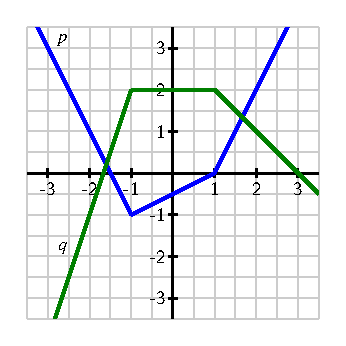
\includegraphics{figures/2_1_Ez3.eps}
\caption{The graphs of $p$ (in blue) and $q$ (in green).} \label{F:2.5.Ez3}
\end{center}
\end{figure}
\ba
	\item Let $C(x) = p(q(x))$.  Determine $C'(0)$ and $C'(3)$.
	\item Find a value of $x$ for which $C'(x)$ does not exist.  Explain your thinking.
	\item Let $Y(x) = q(q(x))$ and $Z(x) = q(p(x))$.  Determine $Y'(-2)$ and $Z'(0)$.	
\ea
\item If a spherical tank of radius 4 feet has $h$ feet of water present in the tank, then the volume of water in the tank is given by the formula
$$V = \frac{\pi}{3} h^2(12-h).$$
\ba
	\item At what instantaneous rate is the volume of water in the tank changing with respect to the \emph{height} of the water at the instant $h = 1$?  What are the units on this quantity?
	\item Now suppose that the height of water in the tank is being regulated by an inflow and outflow (e.g., a faucet and a drain) so that the height of the water at time $t$ is given by the rule $h(t) = \sin(\pi t) + 1$, where $t$ is measured in hours (and $h$ is still measured in feet).  At what rate is the height of the water changing with respect to time at the instant $t = 2$?
	\item Continuing under the assumptions in (b), at what instantaneous rate is the volume of water in the tank changing with respect to \emph{time} at the instant $t = 2$?  
	\item What are the main differences between the rates found in (a) and (c)?  Include a discussion of the relevant units.
\ea
\end{exercises}
\afterexercises 

\clearpage